The detection of the MPS stations is an important part at competition. This chapter gives detailed insights of the new implemented SmartRobotinoDetection component. 


\subsubsection{Overview}

The SmartRobotinoDetection component has only one task: it should detect the MPS stations near by the robot on the field. Therefor, if the component gets triggered, it commands the robot to perform a 360 degree turn and detect all the machines around.

\subsubsection{Old Version 2017}
The former team has implemented the SmartMPSDockingRoboCup component. 

\begin{figure}[h]
\centering
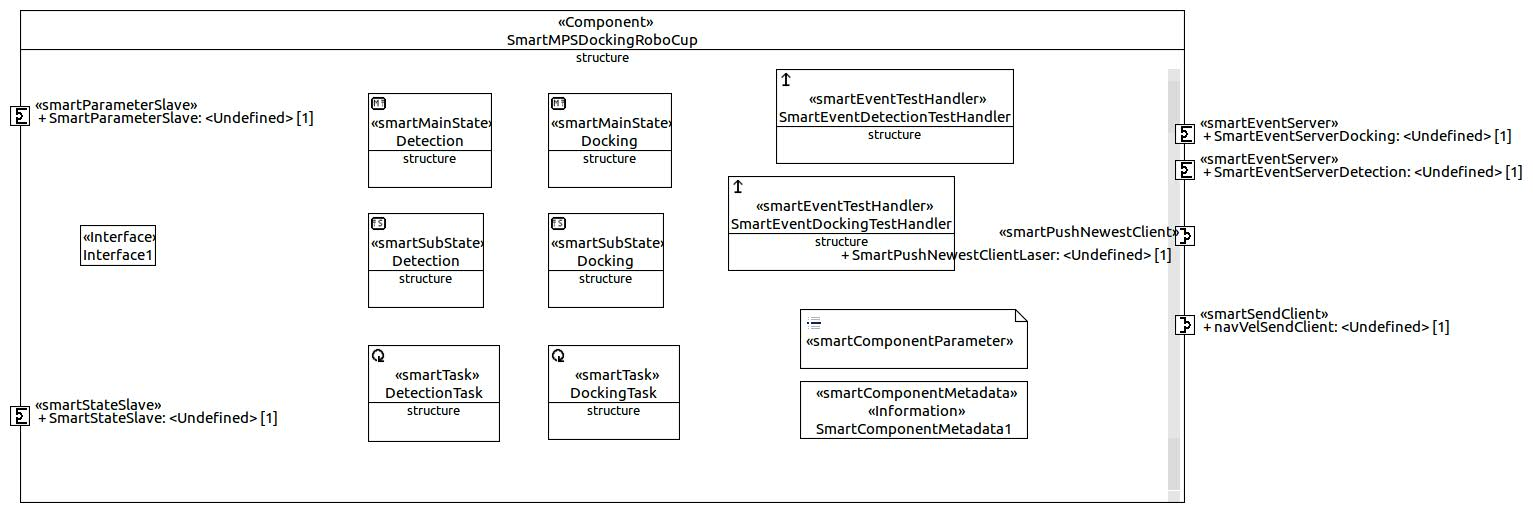
\includegraphics[scale=0.4]{pic/SmartMPSDockingRoboCup.JPG}
\caption{Model of MPS Detection/Docking Component}
\label{fig:i_overview}
\end{figure}

Their idea was to combine the detection of the MPS stations and docking to the stations in one component. The detection worked mostly, but the docking was completely random. This chapter just describes the detection part, and the docking is described in the next chapter. 
The combination of different tasks (detection and docking) contradict the idea of Smartsoft where concrete software components recommended. By splitting the detection from the docking, it would also be possible to replace on the fly the detection via the laser scanner by the detection via the camera, mounted on the robot.
Further the old SmartMPSDockingRoboCup component is implemented in a very confusing way and is hard to understand, so the team of 2018 decided to rewrite the component completely and discard the old one.


\subsubsection{ New Version 2018}
The new version of the detection component is ...

